
\documentclass[a4paper, 10pt, english]{article}
% \documentclass{tmarticle}
\usepackage[]{lipsum} 
\usepackage[]{paralist} 
% \definecolor{TMcodeBackground}{RGB}{240, 240, 240}
% \definecolor{TMbulletinBackground}{RGB}{240, 240, 240}


% decent example of doing mathematics and proofs in LaTeX.
% An Incredible degree of information can be found at
% http://en.wikibooks.org/wiki/LaTeX/Mathematics

% Use wide margins, but not quite so wide as fullpage.sty
\marginparwidth 0.5in 
\oddsidemargin 0.25in 
\evensidemargin 0.10in 
\marginparsep 0.25in
\topmargin 0.25in 
\textwidth 6in \textheight 8 in
% That's about enough definitions

\usepackage[final]{pdfpages}
\usepackage{pythonhighlight}
\usepackage{amsmath,amssymb,amsthm}
\usepackage{upgreek}
\usepackage{float}
% \usepackage[norsk]{babel}
\usepackage[utf8]{inputenc}
\usepackage[T1]{fontenc}
\usepackage{enumitem}
\usepackage{gensymb}
\usepackage{graphicx}
\usepackage{adjustbox}

\usepackage{systeme}
\usepackage{mathtools}
\usepackage{verbatim}
\usepackage{amsfonts}
\usepackage{geometry}
\usepackage{minted}
\usepackage{listings}

% \vec for bold font vector notation
\let\vec\mathbf

% Default fixed font does not support bold face
\DeclareFixedFont{\ttb}{T1}{txtt}{bx}{n}{12} % for bold
\DeclareFixedFont{\ttm}{T1}{txtt}{m}{n}{12}  % for normal

% Custom colors
\usepackage{color}
\definecolor{deepblue}{rgb}{0,0,0.5}
\definecolor{deepred}{rgb}{0.6,0,0}
\definecolor{deepgreen}{rgb}{0,0.5,0}
\definecolor{codegray}{rgb}{0.5,0.5,0.5}
\definecolor{codepurple}{rgb}{0.58,0,0.82}
\definecolor{backcolour}{rgb}{0.95,0.95,0.92}

% Python style for highlighting
\lstdefinestyle{pythonstyle}{
	language=Python,
	basicstyle=\small,
	otherkeywords={self},             % Add keywords here
	keywordstyle=\small\color{deepblue},
	emph={MyClass,__init__},          % Custom highlighting
	emphstyle=\small\color{deepred},    % Custom highlighting style
	stringstyle=\color{deepgreen},
	frame=tb,                         % Any extra options here
	showstringspaces=false            % 
}

\lstdefinestyle{mystyle}{
    backgroundcolor=\color{backcolour},   
    commentstyle=\color{codegreen},
    keywordstyle=\color{magenta},
    numberstyle=\tiny\color{codegray},
    stringstyle=\color{codepurple},
    basicstyle=\footnotesize,
    breakatwhitespace=false,         
    breaklines=true,                 
    captionpos=b,                    
    keepspaces=true,                 
    numbers=left,                    
    numbersep=5pt,                  
    showspaces=false,                
    showstringspaces=false,
    showtabs=false,                  
    tabsize=2
}

% define custom rcases
% \newenvironment{rcases}
%   {\left.\begin{aligned}}
%   {\end{aligned}\right\rbrace}

\lstset{style=pythonstyle,
	breaklines=true}

\usepackage{varioref}
\usepackage{hyperref}
\usepackage[capitalize, noabbrev]{cleveref}

\begin{document}
\author{Jonas Øren}
\title{Mandatory assignment 2, STK2100}
\maketitle

\begin{itemize}

\item [Problem 1]
    \begin{enumerate}
	\item[$(a)$] 
	    Only figure $A$ could have been produced by a regression tree, because the process
	    recursively divides the space into new regions, by dividing previous regions into
	    two new ones, where the dividing line is parallel to the axis of a predictor.
	    This produces areas that are strictly rectangles.

	    - Figure $C$ contains a line that is not parallel to any axis.

	    - Figure $B$ and $D$ have regions that are not rectangles.

	\item[$(b)$] 
	    \begin{figure}[H]
		\centering
		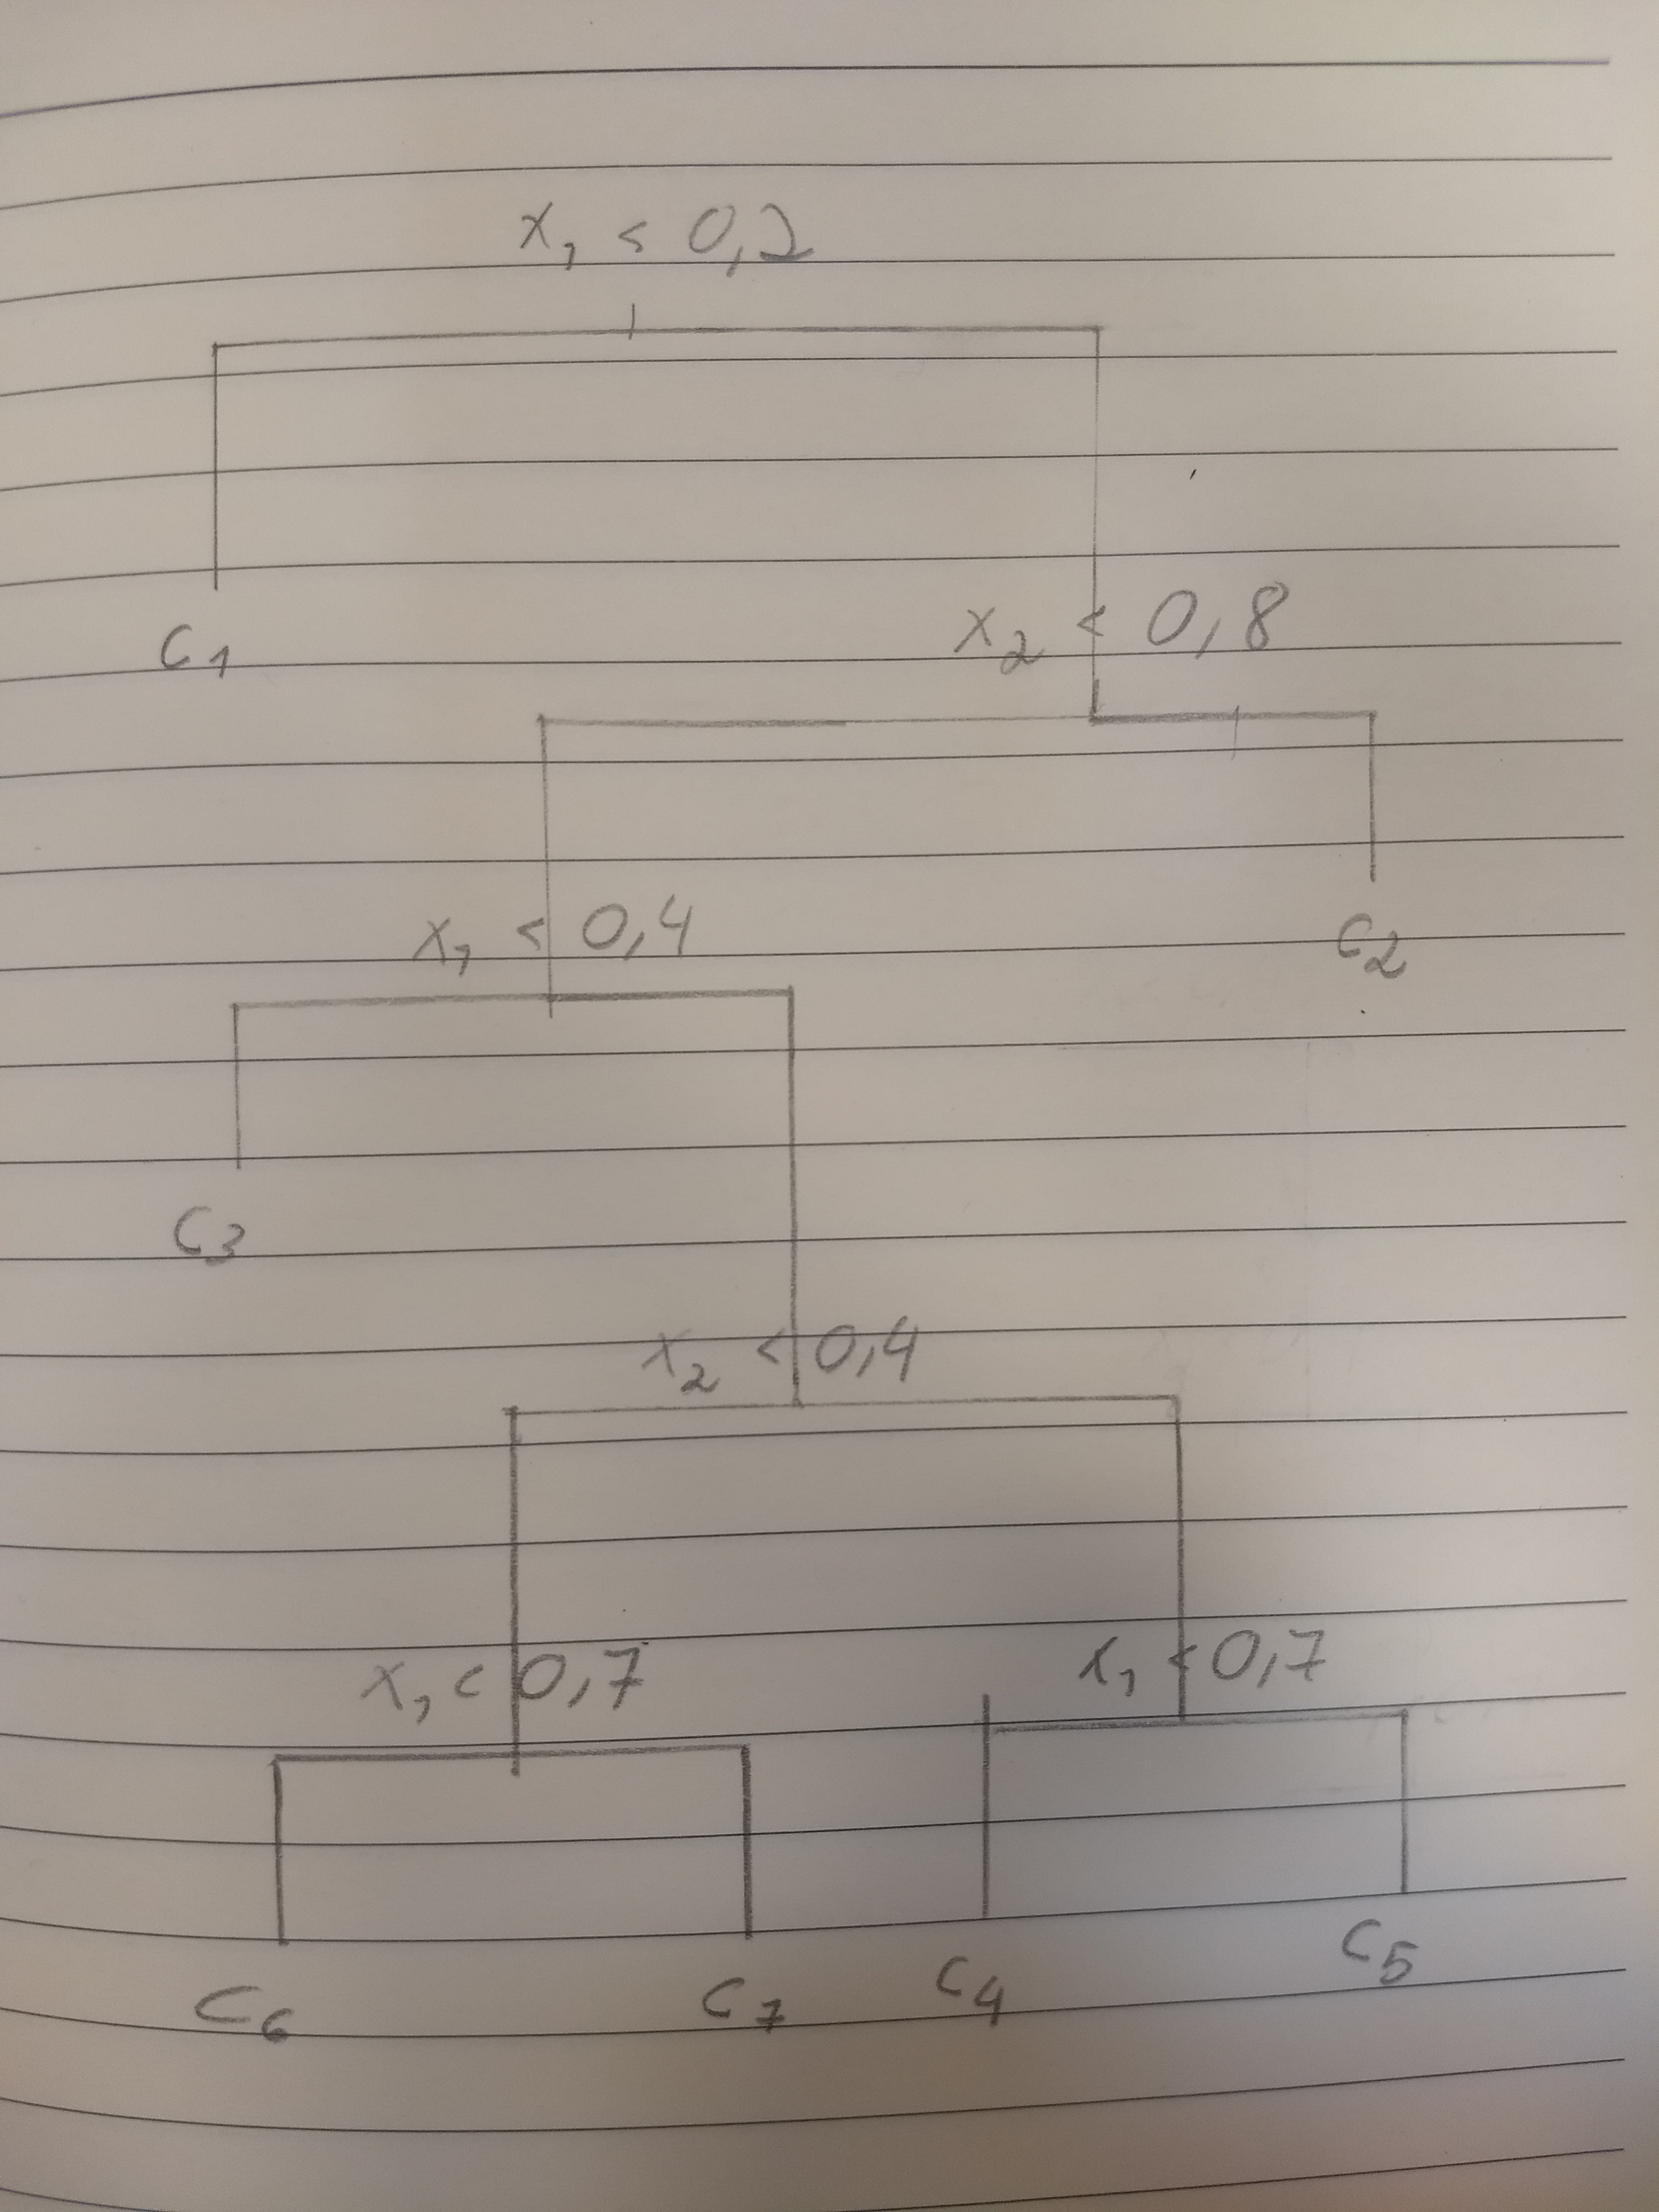
\includegraphics[width=0.6\linewidth]{r-script/plots/tree0.jpg}
		\caption{Sketch of the tree.}
		\label{fig:tree0}
	    \end{figure}
	    The regression tree is shown in \vref{fig:tree0}:


	\item[$(c)$] 
	    The estimates are:
	    \begin{itemize}
		\item[$(i)$] $f(x_1 = 0.5, x_2=0.5) \quad=  c_4$
		\item[$(ii)$] $f(x_1 = 0.3, x_2=0.5) \quad=  c_3$
		\item[$(iii)$] $f(x_1 = 0.5, x_2=0.3) \quad=  c_6$
		\item[$(iv)$] $f(x_1 = 0.95, x_2=0.05)  =  c_7$
		\item[$(v)$] $f(x_1 = 0.05, x_2=0.95)  =  c_1$
		\item[$(vi)$] $f(x_1 = 0.45, x_2=0.75)  =  c_4$
	    \end{itemize}
    \end{enumerate}

\vspace{0.5cm}
\item [Problem 2]

    \begin{enumerate}
	\vspace{0.5cm}
	\item[$(a)$] 
	    \begin{figure}[H]
		\centering
		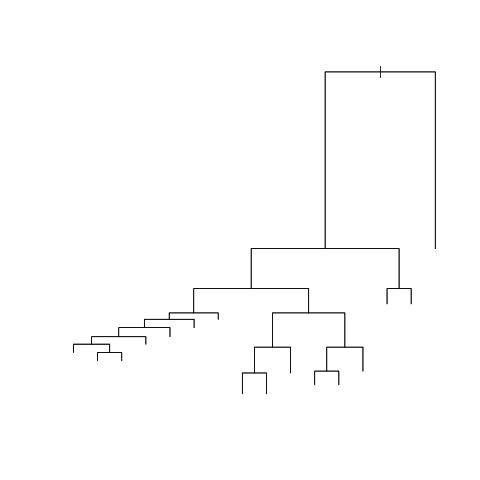
\includegraphics[width=0.6\linewidth]{r-script/plots/unpruned-tree.jpg}
		\caption{Tree before pruning.}
		\label{fig:tree1}
	    \end{figure}
	    \begin{figure}[H]
		\centering
		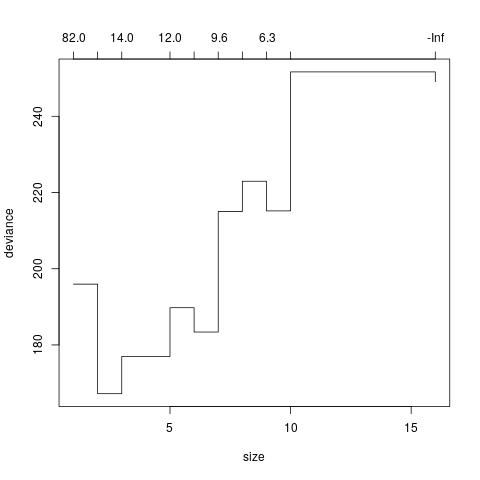
\includegraphics[width=0.6\linewidth]{r-script/plots/deviance.jpg}
		\caption{Deviance vs complexity, found with cross-validation.}
		\label{fig:dev1}
	    \end{figure}
	    \begin{figure}[H]
		\centering
		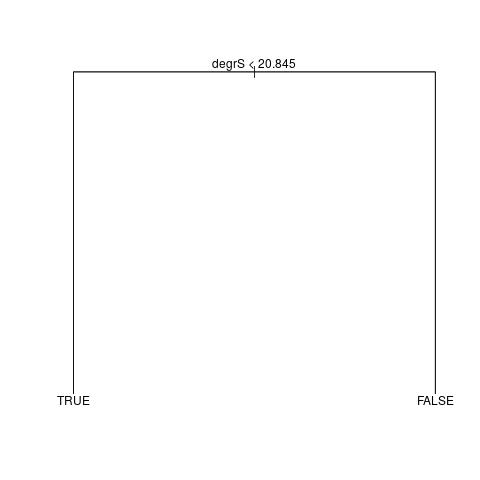
\includegraphics[width=0.6\linewidth]{r-script/plots/tree2.jpg}
		\caption{Tree after pruning.}
		\label{fig:tree2}
	    \end{figure}
	    I set healthy patients as ''TRUE'' and sick patients sa ''FALSE''.
	    I then divide the data into healthy and unhealthy patients, then divide both into test and
	    training data, and the training data into a grow and
	    pruning set, and finally combine the sets of healthy and unhealthy patients.
	    I first grow a tree on the grow set without any restrictions. \vref{fig:tree1} shows the
	    result.

	\item[$(b)$] 
	    Using cross validation i find the relationship between deviance and tree size shown
	    in \vref{fig:dev1}.

	    I then prune the tree (now based on misclassification error, and using the pruning
	    data) and get the decision
	    tree shown in \vref{fig:tree2}

	    \newpage
	\item[$(c)$] 
	    I compute the misclassification errors to be
	    \begin{python}
> err.original
[1] 0.2427184
> err.pruned
[1] 0.2330097
	    \end{python}
	    The pruned tree now does slightly better than the original, but still the
	    improvement is not great, and the model still misclassified almost every fourth
	    observation.

	    The dataset is not very large, and I did not expect classification of disease based on risk
	    factors to be very precise but I did expect the difference in performance between the simpler
	    model and the complex model to be bigger, especially since such a big difference in
	    complexity was chosen.

	\item[$(d)$] 

	    Applying LDA and QDA gives the following prediction errors:
	    \begin{python}
> err.lda
[1] 0.1650485
> err.qda
[1] 0.184466
	    \end{python}
	    In this case the less complex LDA model gives the best predictions on the training
	    set. And LDA also performs better than classification trees.

	
	    \begin{minipage}{\textwidth}
	    \item[$(e)$ ]
		With three classes i get the unpruned tree shown in \vref{fig2:tree1}, deviance
		found with cross validation shown in \vref{fig2:dev1} and the pruned tree
		shown in \vref{fig2:tree2}. The cross-selection only chooses one node, and never predicts the
		third class.

		Computed errors using all four methods are:
		\begin{python}
> err.original
[1] 0.2038835
> err.pruned
[1] 0.1941748
> err.lda
[1] 0.1165049
> err.qda
[1] 0.1359223
		\end{python}
		With more classes the performance is better in this case, but subsequent runs
		show that the errors vary widely from run to run, and I should not infer too
		much from one run.
		But LDA still consistently performs best of all the models.
	    \end{minipage}

	    \begin{figure}[H]
		\centering
		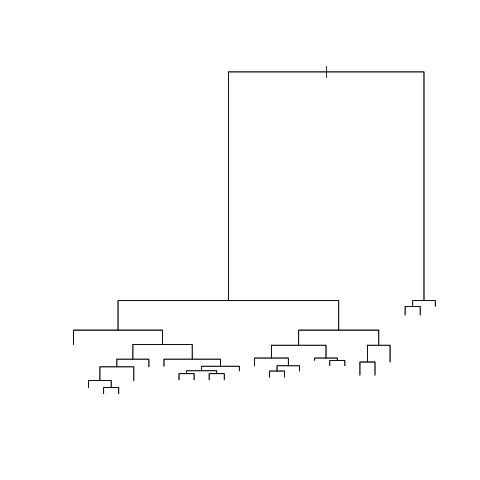
\includegraphics[width=0.6\linewidth]{r-script/plots2/unpruned-tree.jpg}
		\caption{Tree before pruning.}
		\label{fig2:tree1}
	    \end{figure}

	    \begin{figure}[H]
		\centering
		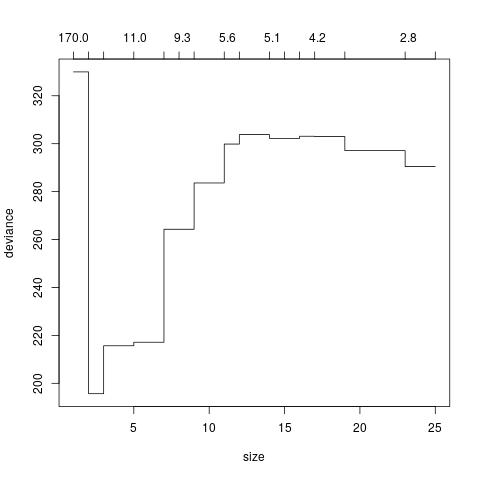
\includegraphics[width=0.6\linewidth]{r-script/plots2/deviance.jpg}
		\caption{Deviance vs tree-complexity with three classes, found with cross-validation.}
		\label{fig2:dev1}
	    \end{figure}

	    \begin{minipage}{\textwidth}
	    \item[$(f)$]
		Report:

		You can use the tree found in \vref{fig:tree2} to classify if a patient is sick or
		healthy by starting at the root of the tree and following the nodes downwards until
		you reach a prediction for the patients health. At each note you go left if the
		statement is true, e.g. at the root node go left if ''degrS < 15.155''. The
		prediction ''TRUE'' means the patient is healthy.
	    \end{minipage}

	    \begin{figure}[H]
		\centering
		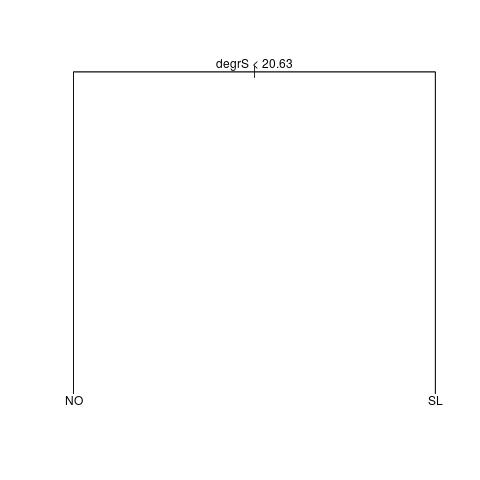
\includegraphics[width=0.6\linewidth]{r-script/plots2/tree2.jpg}
		\caption{Tree after pruning.}
		\label{fig2:tree2}
	    \end{figure}

    \end{enumerate}

    \begin{samepage}
    \item [Problem 3]

	A plot of all fitted models are shown in \vref{fig3:fitted_models}.
	\begin{itemize}

	    \item[$(a)$]
		I randomly split the data into a training set, and a test set of equal size. I then
		randomly split the training set into 5 equal parts and find the optimal number of neighbors
		for the kNN algorithm using 5-fold cross validation.

		I find the optimal k to be 6. \vref{fig3:k_opt} shows the cross validation mean squared error for each
		k. 
		% \vref{fig3:knn} shows the model fitted to the training data.
		Because the data follows a very strong pattern, the algorithm chose a small
		number for k, meaning each point is chosen according to the 6 points nearest
		the chosen point, resulting in a funciton that follows the pattern in the data
		closely.


		\vspace{0.2cm}

	    \item[$(b)$]
		Again using 5-fold cross-validation, I narrow down an interval for lambda, and
		find an optimal lambda close to 5e-5, meaning almost no smoothing is applied to
		the function. Again this is because there is such a strong pattern apparent in
		the data, that the estimated function wants to follow it closely.
		
		\vref{fig3:lambda_opt} shows the cross validation mean squared
		error for each lambda in the narrowed down interval.

		\vspace{0.3cm}
		There is very little difference between the smoothing spline and the
		non-penalized spline model, but I had expected there to be even less difference
		as the smoothing parameter is so close to zero that its effect is negligible.
		I would have expected the smoothing spline to essentially take the same
		form as a non-penalized cubic spline.
    \end{samepage}

		\begin{minipage}{\textwidth}

	    \item[$(c)$]
		The mean squared prediction error for the three models on the test set is:
		    \begin{python}
$`kNN model`
[1] 86.09558

$`Non penalized cubic spline`
[1] 78.44606

$`Smoothing spline`
[1] 83.95698
		    \end{python}

		    The non penalized spline performed the best, but the difference between the
		    prediction errors are small, and I would expect some variability in
		    prediction errors from dataset to dataset, so the models seem to predict
		    about equally well.
		
		\end{minipage}

		\begin{figure}[H]
		    \centering
		    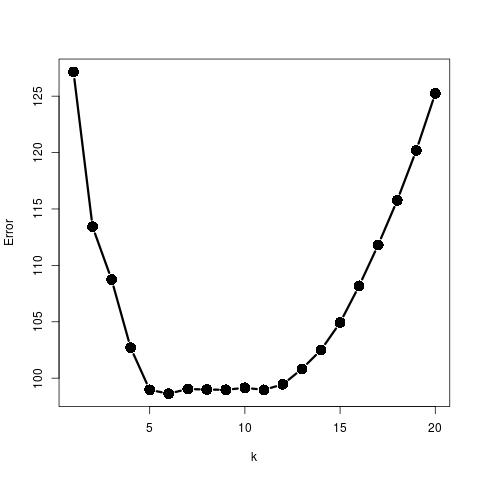
\includegraphics[width=0.6\linewidth]{r-script/plots3/k_opt.jpg}
		    \caption{Cross validation error for each k.}
		    \label{fig3:k_opt}
		\end{figure}
		% \begin{figure}[H]
		%     \centering
		%     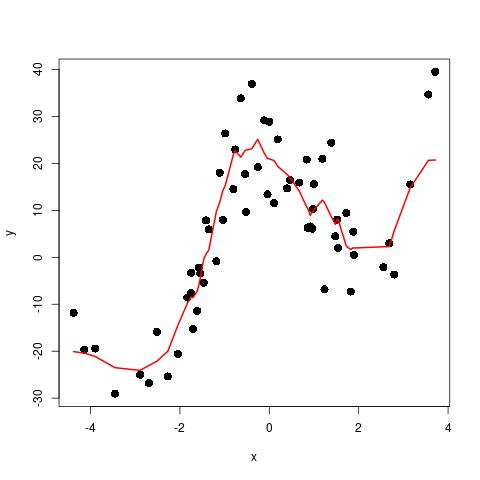
\includegraphics[width=0.6\linewidth]{r-script/plots3/knn.jpg}
		%     \caption{Training points and curve estimated by kNN algorithm.}
		%     \label{fig3:knn}
		% \end{figure}
		\begin{figure}[H]
		    \centering
		    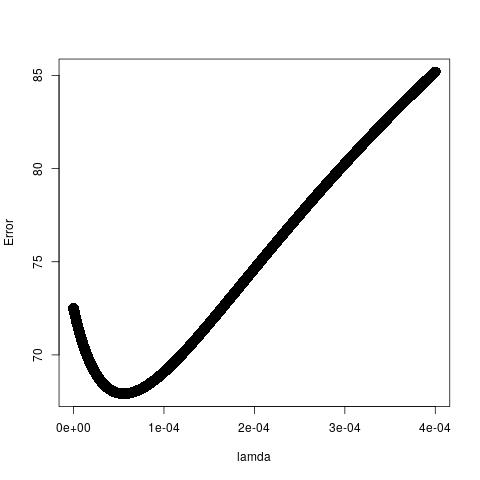
\includegraphics[width=0.6\linewidth]{r-script/plots3/lambda_opt.jpg}
		    \caption{Cross validation error for each lambda.}
		    \label{fig3:lambda_opt}
		\end{figure}
		\begin{figure}[H]
		    \centering
		    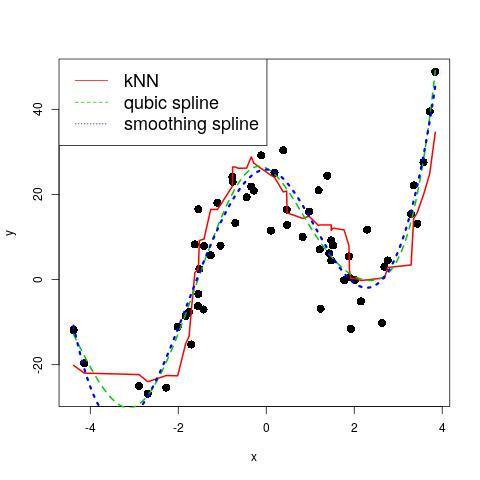
\includegraphics[width=0.6\linewidth]{r-script/plots3/fitted_models.jpg}
		    \caption{Training points and fitted models.}
		    \label{fig3:fitted_models}
		\end{figure}
	\end{itemize}
\end{itemize}
\end{document}
